\chapter{Especificación de la arquitectura}

\section{Arquitectura del sistema}
La arquitectura del sistema se divide en tres partes o subsistemas, cada subsistema tiene una tarea diferenciada dentro del sistema, se puede encontrar una relación entre cada subsistema y las diferentes fases del proceso ETL. Los subsistemas son los siguientes:

\begin{itemize}
	\item \textit{Subsistema de recolección y envío}: Está compuesto de dos módulos, el de recolección y el de envío. El módulo de recolección se encarga de recoger los eventos en el dispositivo ubicuo. El módulo de envío se encarga de enviar los eventos recogidos por el módulo de recolección al módulo de recepción del subsistema de recepción e ingesta.
	
	\item \textit{Subsistema de recepción e ingesta}: Está compuesto por dos módulos, el de recepción y el de ingesta. El módulo de recepción se encarga de centralizar la ingesta de eventos a un único punto de entrada y  de recibir los eventos que le envía el módulo de envío. El módulo de ingesta se encarga de recibir los eventos del módulo de recepción y almacenarlos como mínimo hasta que el módulo de transformación los consuma.

	\item \textit{Subsistema de transformación}:  Está compuesto por dos módulos, el de transformación y el de almacenamiento. El módulo de transformación se encarga de transformar los eventos que consume del módulo de ingesta y de enviarlos al módulo de almacenamiento. El módulo de almacenamiento recibe los eventos transformados del módulo de transformación y los almacena.
\end{itemize}

\subsection{Vista parcial de la arquitectura}
En la figura \ref{fig:arqparcial} se puede ver como se relacionan los subsistemas y los módulos del sistema. Las flechas indican el sentido del flujo de datos.

\begin{figure}[!htb]
	
	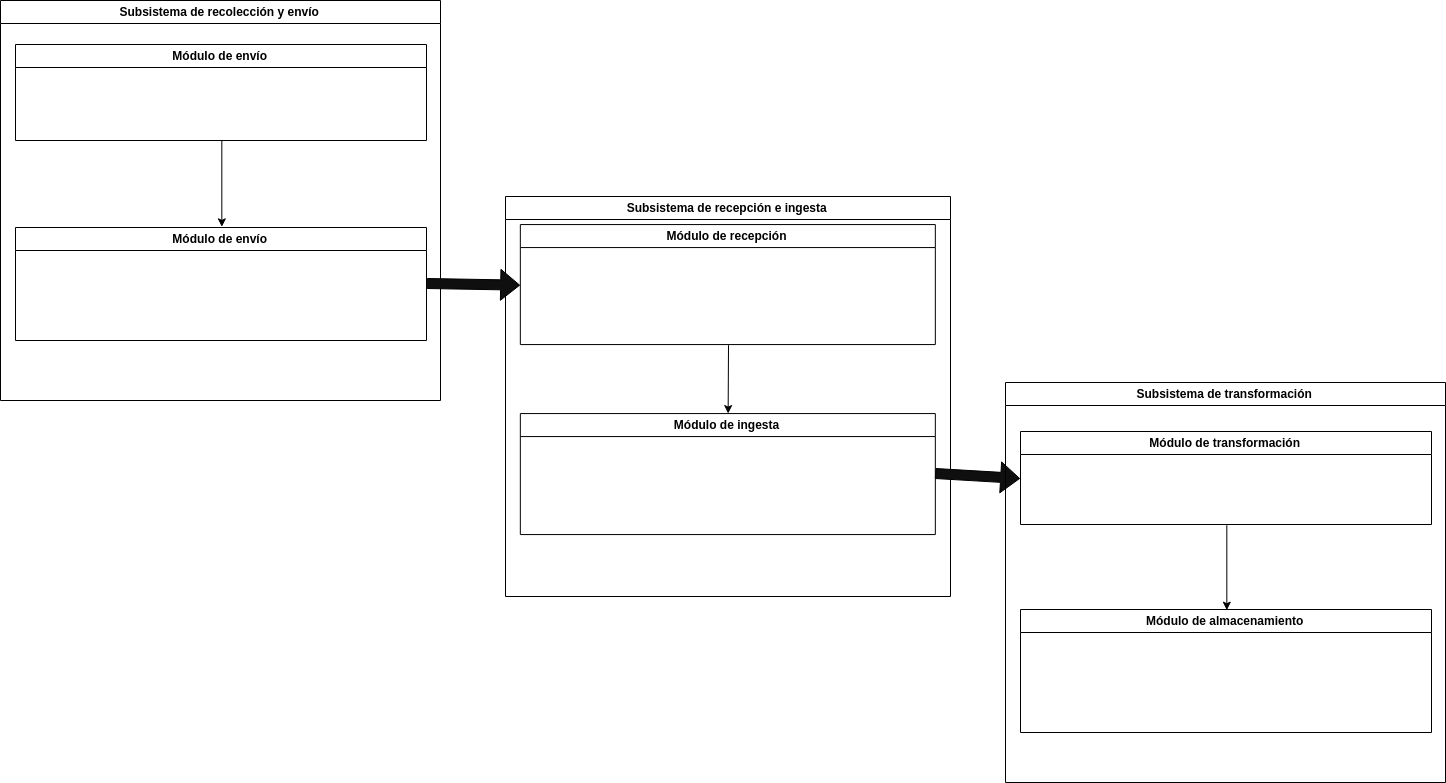
\includegraphics[width=\linewidth] {Moduloss-arquitecturaparcial.png}
	\caption{Vista parcial de la arquitectura del sistema}
	\label{fig:arqparcial}
\end{figure}

\section{Integración con el entorno}
El sistema se ha de integrar con JIRA y con Elastic Search. De la integración con JIRA se espera que el sistema sea capaz de crear un ticket en JIRA con información obtenida de los eventos. De la integración con Elastic Search se espera que el sistema sea capaz de publicar información, obtenida de las alertas, en un índice de Elastic Search con el objetivo de que la información publicada sea visible en Kibana.
